\documentclass[journal,12pt,twocolumn]{IEEEtran}

\usepackage{setspace}
\usepackage{gensymb}
\singlespacing
\usepackage[cmex10]{amsmath}
\usepackage{multirow}
\usepackage{amsthm}
\usepackage{mathrsfs}
\usepackage{txfonts}
\usepackage{stfloats}
\usepackage{bm}
\usepackage{cite}
\usepackage{cases}
\usepackage{subfig}

\usepackage{longtable}

\usepackage{enumitem}
\usepackage{mathtools}
\usepackage{steinmetz}
\usepackage{tikz}
\usepackage{circuitikz}
\usepackage{verbatim}
\usepackage{tfrupee}
\usepackage[breaklinks=true]{hyperref}
\usepackage{graphicx}
\usepackage{tkz-euclide}

\usetikzlibrary{calc,math}
\usepackage{listings}
    \usepackage{color}                                            %%
    \usepackage{array}                                            %%
    \usepackage{longtable}                                        %%
    \usepackage{calc}                                             %%
    \usepackage{multirow}                                         %%
    \usepackage{hhline}                                           %%
    \usepackage{ifthen}                                           %%
    \usepackage{lscape}     
\usepackage{multicol}
\usepackage{chngcntr}

\DeclareMathOperator*{\Res}{Res}

\renewcommand\thesection{\arabic{section}}
\renewcommand\thesubsection{\thesection.\arabic{subsection}}
\renewcommand\thesubsubsection{\thesubsection.\arabic{subsubsection}}

\renewcommand\thesectiondis{\arabic{section}}
\renewcommand\thesubsectiondis{\thesectiondis.\arabic{subsection}}
\renewcommand\thesubsubsectiondis{\thesubsectiondis.\arabic{subsubsection}}


\hyphenation{op-tical net-works semi-conduc-tor}
\def\inputGnumericTable{}                                 %%

\lstset{
%language=C,
frame=single, 
breaklines=true,
columns=fullflexible
}
\graphicspath{{./Figures/}}
\begin{document}


\newtheorem{theorem}{Theorem}[section]
\newtheorem{problem}{Problem}
\newtheorem{proposition}{Proposition}[section]
\newtheorem{lemma}{Lemma}[section]
\newtheorem{corollary}[theorem]{Corollary}
\newtheorem{example}{Example}[section]
\newtheorem{definition}[problem]{Definition}

\newcommand{\BEQA}{\begin{eqnarray}}
\newcommand{\EEQA}{\end{eqnarray}}
\newcommand{\define}{\stackrel{\triangle}{=}}
\bibliographystyle{IEEEtran}
\raggedbottom
\setlength{\parindent}{0pt}
\providecommand{\mbf}{\mathbf}
\providecommand{\pr}[1]{\ensuremath{\Pr\left(#1\right)}}
\providecommand{\qfunc}[1]{\ensuremath{Q\left(#1\right)}}
\providecommand{\sbrak}[1]{\ensuremath{{}\left[#1\right]}}
\providecommand{\lsbrak}[1]{\ensuremath{{}\left[#1\right.}}
\providecommand{\rsbrak}[1]{\ensuremath{{}\left.#1\right]}}
\providecommand{\brak}[1]{\ensuremath{\left(#1\right)}}
\providecommand{\lbrak}[1]{\ensuremath{\left(#1\right.}}
\providecommand{\rbrak}[1]{\ensuremath{\left.#1\right)}}
\providecommand{\cbrak}[1]{\ensuremath{\left\{#1\right\}}}
\providecommand{\lcbrak}[1]{\ensuremath{\left\{#1\right.}}
\providecommand{\rcbrak}[1]{\ensuremath{\left.#1\right\}}}
\theoremstyle{remark}
\newtheorem{rem}{Remark}
\newcommand{\sgn}{\mathop{\mathrm{sgn}}}
\providecommand{\abs}[1]{\left\vert#1\right\vert}
\providecommand{\res}[1]{\Res\displaylimits_{#1}} 
\providecommand{\norm}[1]{\left\lVert#1\right\rVert}
%\providecommand{\norm}[1]{\lVert#1\rVert}
\providecommand{\mtx}[1]{\mathbf{#1}}
\providecommand{\mean}[1]{E\left[ #1 \right]}
\providecommand{\fourier}{\overset{\mathcal{F}}{ \rightleftharpoons}}
%\providecommand{\hilbert}{\overset{\mathcal{H}}{ \rightleftharpoons}}
\providecommand{\system}{\overset{\mathcal{H}}{ \longleftrightarrow}}
	%\newcommand{\solution}[2]{\textbf{Solution:}{#1}}
\newcommand{\solution}{\noindent \textbf{Solution: }}
\newcommand{\cosec}{\,\text{cosec}\,}
\providecommand{\dec}[2]{\ensuremath{\overset{#1}{\underset{#2}{\gtrless}}}}
\newcommand{\myvec}[1]{\ensuremath{\begin{pmatrix}#1\end{pmatrix}}}
\newcommand{\mydet}[1]{\ensuremath{\begin{vmatrix}#1\end{vmatrix}}}
\newcommand*{\permcomb}[4][0mu]{{{}^{#3}\mkern#1#2_{#4}}}
\newcommand*{\perm}[1][-3mu]{\permcomb[#1]{P}}
\newcommand*{\comb}[1][-1mu]{\permcomb[#1]{C}}
\numberwithin{equation}{subsection}
\makeatletter
\@addtoreset{figure}{problem}
\makeatother
\let\StandardTheFigure\thefigure
\let\vec\mathbf
\renewcommand{\thefigure}{\theproblem}
\def\putbox#1#2#3{\makebox[0in][l]{\makebox[#1][l]{}\raisebox{\baselineskip}[0in][0in]{\raisebox{#2}[0in][0in]{#3}}}}
     \def\rightbox#1{\makebox[0in][r]{#1}}
     \def\centbox#1{\makebox[0in]{#1}}
     \def\topbox#1{\raisebox{-\baselineskip}[0in][0in]{#1}}
     \def\midbox#1{\raisebox{-0.5\baselineskip}[0in][0in]{#1}}
\vspace{3cm}
\title{Assignment 5}
\author{Sujal - AI20BTECH11020}
\maketitle
\newpage
\bigskip
\renewcommand{\thefigure}{\theenumi}
\renewcommand{\thetable}{\theenumi}
Download all python codes from 
\begin{lstlisting}
https://github.com/sujal100/Probability_and_Random_variable/tree/main/exercise_5/codes
\end{lstlisting}

and latex codes from 

\begin{lstlisting}
https://github.com/https://github.com/sujal100/Probability_and_Random_variable/blob/main/exercise_5/exercise_5_main_tex.tex
\end{lstlisting}
\section{Problem [GATE(2003)EC-61]}
Let $X$ and $Y$ be two statistically independent random variables uniformly
distributed in the ranges $(-1,1)$ and $(-2,1)$ respectively. Let $Z = X + Y.$ then the probability that $[Z\leq-2]$ is\\
(a) zero
(b)$\dfrac{1}{6}$
(c)$\dfrac{1}{3}$
(d)$\dfrac{1}{12}$
\section{Solution}
Let be the probability densities of random variables $X ,Y $and $Z.$ \\
\begin{align}
    p_X\brak{x} &= \Pr\brak{X=x} \\
    p_Y\brak{y} &= \Pr\brak{Y=y}  \\
    p_Z\brak{z} &= \Pr\brak{Z=z}
\end{align}
The pdf of $Z(=X+Y)$ will be convolution of pdf of $X$ and pdf of $Y$ as shown below.


\tikzset{every picture/.style={line width=0.5pt}} %set default line width to 0.75pt        

\begin{tikzpicture}[x=0.45pt,y=0.5pt,yscale=-1,xscale=1]
%uncomment if require: \path (0,300); %set diagram left start at 0, and has height of 300

%Straight Lines [id:da7994322016020907] 
\draw [line width=0.75]    (65.3,280.6) -- (580.3,280.6) ;
%Straight Lines [id:da6298726397789813] 
\draw [line width=0.75]    (321.8,68.4) -- (322.8,280.6) ;
%Shape: Right Angle [id:dp8023791863547924] 
\draw  [color={rgb, 255:red, 0; green, 0; blue, 0 }  ,draw opacity=1 ][line width=1.5]  (254.8,168.6) -- (389.8,168.6) -- (389.8,279) ;
%Straight Lines [id:da07001326664875096] 
\draw [line width=1.5]    (254.8,168.6) -- (254.8,279) ;

% Text Node
\draw (403,152.4) node [anchor=north west][inner sep=0.75pt]    {$\dfrac{1}{2}$};
% Text Node
\draw (240,285.4) node [anchor=north west][inner sep=0.75pt]    {$-1$};
% Text Node
\draw (385,282.4) node [anchor=north west][inner sep=0.75pt]    {$1$};
% Text Node
\draw (318,283.4) node [anchor=north west][inner sep=0.75pt]    {$0$};
% Text Node
\draw (303,44.4) node [anchor=north west][inner sep=0.75pt]    {$f_{x}( x)$};
% Text Node
\draw (590,269.4) node [anchor=north west][inner sep=0.75pt]    {$x$};
\end{tikzpicture}


\tikzset{every picture/.style={line width=0.5pt}} %set default line width to 0.75pt        

\begin{tikzpicture}[x=0.45pt,y=0.5pt,yscale=-1,xscale=1]
%uncomment if require: \path (0,300); %set diagram left start at 0, and has height of 300

%Straight Lines [id:da7994322016020907] 
\draw [line width=0.75]    (65.3,280.6) -- (580.3,280.6) ;
%Straight Lines [id:da6298726397789813] 
\draw [line width=0.75]    (321.8,68.4) -- (322.8,280.6) ;
%Shape: Right Angle [id:dp8023791863547924] 
\draw  [color={rgb, 255:red, 0; green, 0; blue, 0 }  ,draw opacity=1 ][line width=1.5]  (267.8,168.6) -- (389.8,168.6) -- (389.8,279) ;
%Straight Lines [id:da07001326664875096] 
\draw [line width=1.5]    (267.8,168.6) -- (189.8,169.4) -- (189.8,280) ;

% Text Node
\draw (403,152.4) node [anchor=north west][inner sep=0.75pt]    {$\dfrac{1}{3}$};
% Text Node
\draw (240,282.4) node [anchor=north west][inner sep=0.75pt]    {$-1$};
% Text Node
\draw (385,282.4) node [anchor=north west][inner sep=0.75pt]    {$1$};
% Text Node
\draw (318,283.4) node [anchor=north west][inner sep=0.75pt]    {$0$};
% Text Node
\draw (303,44.4) node [anchor=north west][inner sep=0.75pt]    {$f_{y}( y)$};
% Text Node
\draw (590,269.4) node [anchor=north west][inner sep=0.75pt]    {$y$};
% Text Node
\draw (175,280.4) node [anchor=north west][inner sep=0.75pt]    {$-2$};
\end{tikzpicture}

\tikzset{every picture/.style={line width=0.5pt}} %set default line width to 0.75pt        

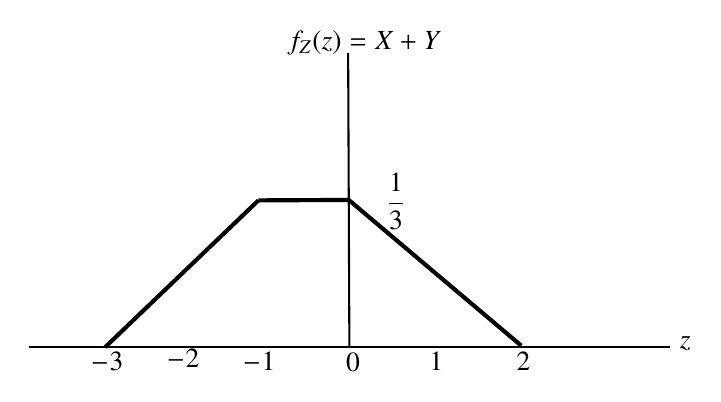
\begin{tikzpicture}[x=0.45pt,y=0.5pt,yscale=-1,xscale=1]
%uncomment if require: \path (0,300); %set diagram left start at 0, and has height of 300

%Straight Lines [id:da7994322016020907] 
\draw [line width=0.75]    (65.3,280.6) -- (580.3,280.6) ;
%Straight Lines [id:da6298726397789813] 
\draw [line width=0.75]    (321.8,68.4) -- (322.8,280.6) ;
%Straight Lines [id:da3048610517318646] 
\draw [line width=1.5]    (249.8,174.8) -- (322.3,174.5) ;
%Straight Lines [id:da21348606992409946] 
\draw [line width=1.5]    (249.8,174.8) -- (126.8,280.8) ;
%Straight Lines [id:da9537386999126634] 
\draw [line width=1.5]    (322.3,174.5) -- (460.8,279.8) ;

% Text Node
\draw (350,153.4) node [anchor=north west][inner sep=0.75pt]    {$\dfrac{1}{3}$};
% Text Node
\draw (236,282.4) node [anchor=north west][inner sep=0.75pt]    {$-1$};
% Text Node
\draw (385,282.4) node [anchor=north west][inner sep=0.75pt]    {$1$};
% Text Node
\draw (318,283.4) node [anchor=north west][inner sep=0.75pt]    {$0$};
% Text Node
\draw (271,50.4) node [anchor=north west][inner sep=0.75pt]    {$f_{Z}( z) =X+Y$};
% Text Node
\draw (175,280.4) node [anchor=north west][inner sep=0.75pt]    {$-2$};
% Text Node
\draw (114,282.4) node [anchor=north west][inner sep=0.75pt]    {$-3$};
% Text Node
\draw (455,282.4) node [anchor=north west][inner sep=0.75pt]    {$2$};
% Text Node
\draw (586,271.4) node [anchor=north west][inner sep=0.75pt]    {$z$};
\end{tikzpicture}
Now
$$
\begin{aligned}
p[Z \leq z] &=\int_{-\infty}^{z} f_{Z}(z) d z \\
p[Z \leq-2] &=\int_{-\infty}^{-2} f_{Z}(z) d z \\
&=\text { Area }[z \leq-2] \\
&=\frac{1}{2} \times \frac{1}{6} \times 1=\frac{1}{12}
\end{aligned}
$$
Hence $(\mathrm{D})$ is correct option.
\end{document}